Pendant ce stage, j'ai également cherché à compléter l'ensemble des lois de commutation.

J'ai choisi comme critère de complétude le fait que tous les couples de fonctions
du langage (tous les cas de figure possibles où l'on pourrait vouloir commuter
deux fonctions) soient envisagés.

\begin{figure}
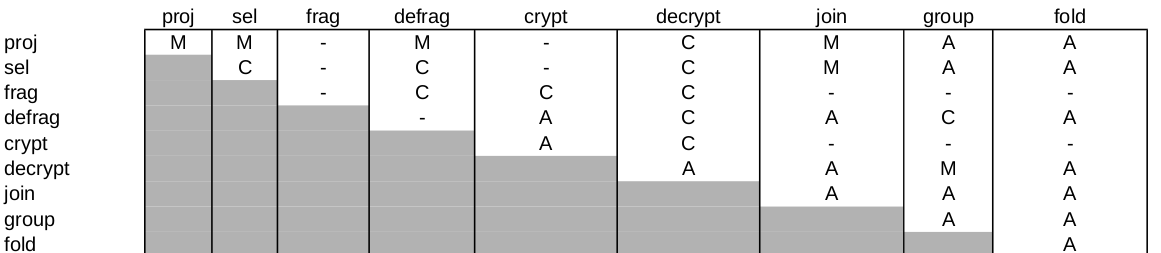
\includegraphics[width=\textwidth]{complLoisBilan.png}
\caption{Bilan des lois conservées (C), modifiées (M) et ajoutées (A)}
\label{complLois}
\end{figure}

Le tableau de la figure \ref{complLois}  montre quelles lois étaient déjà
présentes dans la thèse de 2016 ou dans l'article de 2015 de R. Cherrueau
et ont été conservées (marquées avec un \emph{C}),
quelles lois nous avons modifiées (marquées avec un \emph{M}),
quelles lois nous avons rajoutées (marquées avec un \emph{A})
et quelles lois n'ont pas à être considérées dans l'approche qui est celle
de C2QL (marquées d'un tiret \og - \fg{}).

Pour un document contenant l'ensemble des lois après ce stage,
se référer à l'annexe B.
